\documentclass[a4paper]{article}
\usepackage{amsmath}
\usepackage{hyperref}
\usepackage{enumitem}
\usepackage{graphicx}
\usepackage[utf8]{inputenc}
\usepackage[T1]{fontenc}
\usepackage{textcomp}
\usepackage{gensymb}

\title{Master on Robotics: Perception Systems - Exercise 1.3}
\date{28-10-2015}
\author{Juan Pedro López Cabrera}

\begin{document}
  \pagenumbering{gobble}
  \maketitle

  \newpage
  \pagenumbering{arabic}

  \section{Exercise 3}
Go to the link \url{http://www.ptgrey.com/blackfly-09-mp-color-gige-vision-poe-sony-icx692-camera}, which is a digital camera from one of
the major camera brands used in robotics.
\begin{enumerate}[label=\alph*.]
    \item Try to understand the specs by drawing them in a sketch similar to that of slide 14.

    \begin{figure}[ht]
      \centering
      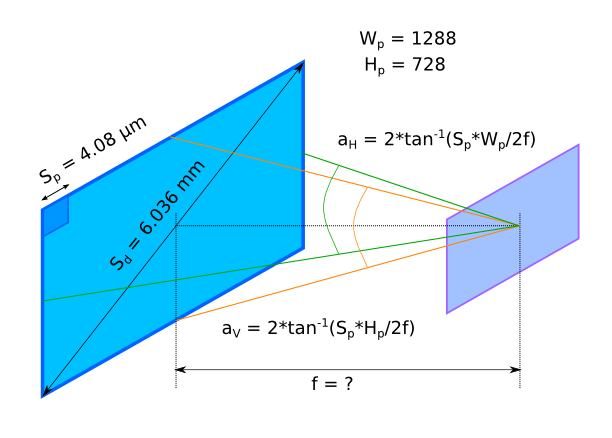
\includegraphics[scale=0.5]{Exercise_1_3_a}
      \caption{Cam specs diagram.}
      \label{fig:cam_specs}
    \end{figure}

\item Using a Lense of 8mm ( \url{http://www.ptgrey.com/m12-micro-lens-8mm-3} ), How many pixels will represent the Mona Lisa painting
if it is situated at 1,2,5,10 m ? Draw a plot distance-pixels. (Mona Lisa dimensions are: 77cm x 53 cm, \url{https://en.wikipedia.
org/wiki/Mona_Lisa} )

The proposed formula to solve this exercise should be divided in two: one for the horizontal pixels and one for the vertical pixels. We'll multiply them later to get the final amount of pixels needed to represent the Mona Lisa.

\begin{equation}
{horizontal\ pixels} = \dfrac {pixel\ width \times width\ of\ the\ Mona\ Lisa }{2 \times distance \times \tan{(0.5 \times horizontal\ angle)}}
\end{equation}

\begin{equation}
{vertical\ pixels} = \dfrac {pixel\ height \times height\ of\ the\ Mona\ Lisa }{2 \times distance \times \tan{(0.5 \times vertical\ angle)}}
\end{equation}

Given these formulas, we can calculate how many pixels we need to represent the Mona Lisa:

\begin{itemize}
  \item At 1m, 1509 horizontal pixels x 1039 vertical pixels are needed.
  \item At 2m, 754 horizontal pixels x 519 vertical pixels are needed.
  \item At 5m, 301 horizontal pixels x 207 vertical pixels are needed.
  \item At 10m, 150 horizontal pixels x 103 vertical pixels are needed.
\end{itemize}

\begin{figure}[ht]
  \centering
  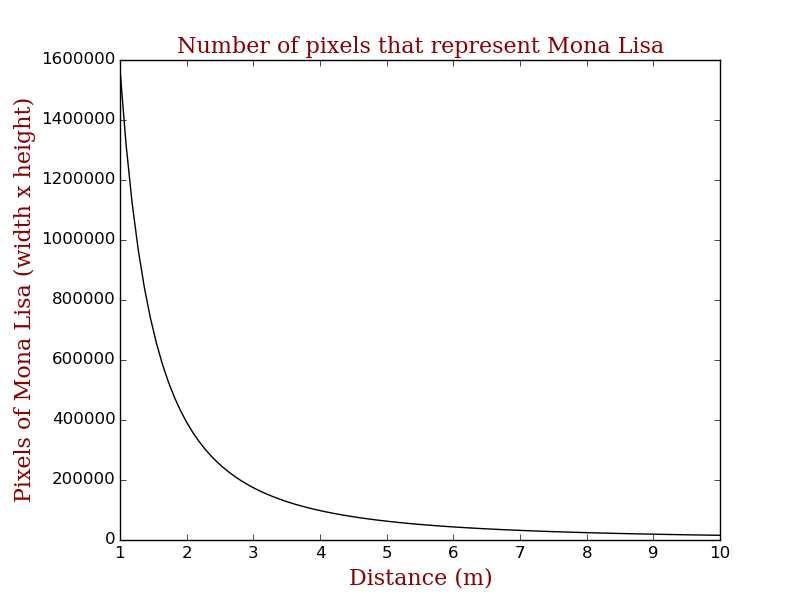
\includegraphics[scale=0.5]{Exercise_1_3_b}
  \caption{Distance vs pixels plot.}
  \label{fig:mona_lista_pixels_width}
\end{figure}

\newpage
\item Why the proposed (linked) lense in b) could not be used easily with this camera ?

The proposed lens has an S-mount which has an M12 thread, whereas our camera can only use CS and C-mount lenses which have 1 inch threads.

\end{enumerate}

\end{document}
